\section{文档说明}\label{sec:docintro}


本手册由 \textbf{\href{https://cssacph.dk}{哥本哈根中国学生学者联合会（CSSA‑Copenhagen）}} 发起并持续维护，旨在为计划赴丹麦（尤其是哥本哈根地区）求学、交换或工作的同学提供 \textbf{一站式、可协作、可持续更新} 的实用信息。内容涵盖行前准备至在丹生活的方方面面，帮助大家少踩坑、多交流、快速融入～

本手册目前共有共建版和年度版两个版本。\textbf{共建版}手册为在线谷歌文档（链接： \href{https://docs.google.com/document/d/1nDohKDCMP-nRd01MiaQxyaOsbb292zW-y6yi3ryS4jo/edit?usp=sharing}{Google Doc}），欢迎所有热心的朋友分享任何在丹麦生活、工作、学习的攻略或经验。学联会定期对文档中的内容进行维护与更新。

\textbf{年度版}手册即为本PDF文档，本文档由学联编辑组整合了共建版的核心内容以及学联在微信公众号及小红书上发布的独家攻略，计划在每学年初或有重大政策变革时进行大版本更新。目前版本为 \textcolor{blue}{\textbf{2025-2026学年版}}。最近更新时间为\textcolor{blue}{\textbf{\today}}。

\begin{grayleftbox} \textbf{免责声明： }
\begin{itemize}
 \item 本手册所载信息均由学联及志愿者根据公开资料、个人经验及官方文件整理，仅供学习交流之用，不构成任何法律、医疗、签证或金融等专业建议。
 \item 由于政策、汇率及服务条款可能随时调整，我们无法保证所有内容始终最新、最完整。使用手册信息前，请务必自行向相关院校、机构及主管部门核实；因依赖本手册内容而产生的任何损失或责任，CSSA-Copenhagen 与作者团队概不承担。
 \item 若发现错误或过期信息，欢迎通过下方联系方式反馈，共同完善手册。
\end{itemize}

\end{grayleftbox}


\vspace{1em}
\textbf{联系我们：} cssa.copenhagen@gmail.com \quad\textbar\quad
欢迎扫码关注 \textcolor{ForestGreen}{\textbf{微信公众号}} \& \textcolor{red}{\textbf{小红书}}

\begin{figure}[H]
  \centering
  \setlength{\tabcolsep}{1em} % 控制两图水平间距
  \begin{tabular}{cc}
    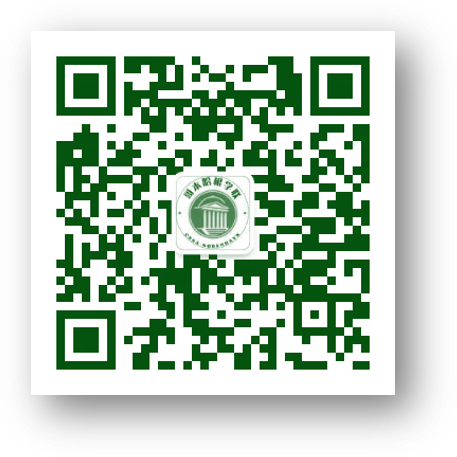
\includegraphics[width=0.26\linewidth]{figures/wechat_qr.png} &
    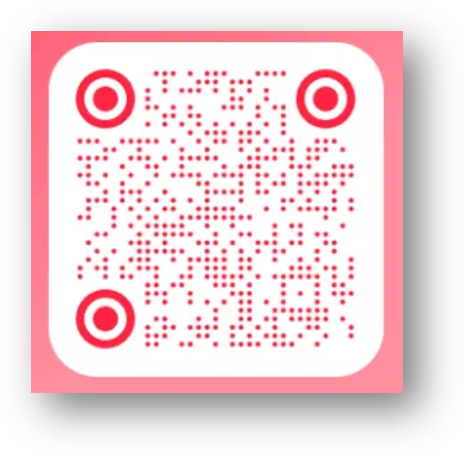
\includegraphics[width=0.26\linewidth]{figures/xiaohongshu_qr.png} \\
    \scriptsize 微信公众号 & \scriptsize 小红书 \\
  \end{tabular}
\end{figure}

\begin{grayleftbox}
\textbf{入群信息: }

若想加入学联 2025 年丹麦留学新生群，可在学联微信公众号 \textbf{【哥本哈根 CSSA】} 或小红书 \textbf{【哥本哈根学联（CSSA）】} 后台私信，获取入群方式。
\end{grayleftbox}


\begin{grayleftbox} \textbf{内容贡献者和编者栏}
\begin{itemize}
 \item \textbf{内容贡献者：} 感谢所有为共建版手册提供内容支持的贡献者。若您希望留下姓名，可联系我们告知，我们将在之后的手册更新中列入您的名字。
 \item \textbf{学联小编（按首字母排序）：} 出门钓鱼让二儿他妈烙了张糖饼但一条鱼没钓上于是去菜市场买了两条说是自己钓上来的二儿他爸、哥哈老油条、猴子、斯特兰奇、Wen、柚子。
\end{itemize}

\end{grayleftbox}